
\documentclass[12pt]{letter}

\usepackage[margin=1in,footskip=0.25in]{geometry}
\usepackage{amsfonts}
\usepackage{amsthm}
\usepackage{pgf}
\usepackage{tikz}
\usepackage{amsmath}
\usetikzlibrary{arrows,automata}
\usetikzlibrary{positioning}
\usepackage[latin1]{inputenc}
\tikzset{>=latex}
\newcommand\tab[1][2cm]{\hspace*{#1}}

\begin{document}

Oct 29, 2017 \\ Viet Tran\\ vtran1@cs.uml.edu\\COMP.3040 Foundation of Computer Science 

\centering Homework III Solution

\flushleft

\begin{enumerate}

%	2.1	%
\item[\textbf{2.1)}]Recall the CFG $G_4$ that we gave in Example 2.4. For convenience, let's rename its variables with single letters as follows.

\setlength\parindent{150pt} $E \rightarrow E + T \mid T $ \\ $T \rightarrow T \times F \mid F $ \\ $F \rightarrow (E)  \mid  a$ \\  \setlength\parindent{0pt}
\leavevmode \\
Give parse trees and derivations of each string.
\begin{enumerate}
	\item[\textbf{a}.] a \\
	The derivation is $E \Rightarrow T \Rightarrow F \Rightarrow a.$
	\begin{center}
	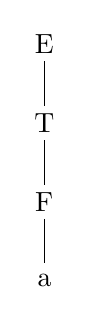
\begin{tikzpicture}[state/.style={inner sep=0pt, minimum size=12pt},node distance=1cm, on grid, auto] 
		\node[state] (q0) {E};
		\node[state] (q1) [below= of q0] {T};
		\node[state] (q2)[below= of q1]  {F};
		\node[state] (q3)[below= of q2]  {a};
		\path[-] 
			(q0) edge node {} (q1)
			(q1) edge node {} (q2)
			(q2) edge node {} (q3);
	\end{tikzpicture}
	\end{center}

	\item[\textbf{b}.] $a + a$ \\
	The derivation is $E \Rightarrow E + T \Rightarrow T + T \Rightarrow F + T \Rightarrow a + T \Rightarrow a + F \Rightarrow a + a.$
	\begin{center}
	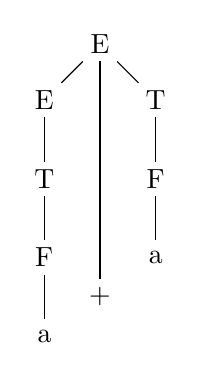
\begin{tikzpicture}[state/.style={inner sep=0pt, minimum size=12pt},node distance=1cm, on grid, auto] 
		\node[state] (q0) {E};
		\node[state] (q1) [below left=of q0] {E};
		\node[state] (q2)[below=of q1]  {T};
		\node[state] (q3)[below=of q2]  {F};
		\node[state] (q4)[below=of q3]  {a};
		\node[state] (q5)[below=3.2cm of q0]  {$+$};
		\node[state] (q6)[below right=of q0]  {T};
		\node[state] (q7)[below=of q6]  {F};
		\node[state] (q8)[below=of q7]  {a};
		\path[-] 
			(q0) edge node {} (q1) edge node {} (q5) edge node {} (q6)
			(q1) edge node {} (q2)
			(q2) edge node {} (q3)
			(q3) edge node {} (q4)
			(q6) edge node {} (q7)
			(q7) edge node {} (q8);
	\end{tikzpicture}
	\end{center}
	\newpage

	\item[\textbf{c}.] $a + a + a$ \\
	The derivation is $E \Rightarrow E + T \Rightarrow E + T + T \Rightarrow T + T + T \Rightarrow F + T + T \Rightarrow a + T+ T \Rightarrow a + F + T \Rightarrow a + a + T \Rightarrow a + a+ F \Rightarrow a + a+ a.$
	\begin{center}
	\begin{tikzpicture}[state/.style={inner sep=0pt, minimum size=12pt},node distance=1cm, on grid, auto] 
		\node[state] (q0) {E};
		\node[state] (q1) [below left=2cm of q0] {E};
		\node[state] (q2) [below left=of q1] {E};
		\node[state] (q3) [below=of q2] {T};
		\node[state] (q4) [below=of q3] {F};
		\node[state] (q5) [below=of q4] {a};
		\node[state] (q6) [below=3.4cm of q1] {$+$};
		\node[state] (q7) [below right =of q1] {T};
		\node[state] (q8) [below=of q7] {F};
		\node[state] (q9) [below=of q8] {a};
		\node[state] (q10) [below=4cm of q0] {$+$};
		\node[state] (q11) [below right=2cm of q0] {T};
		\node[state] (q12) [below=of q11] {F};
		\node[state] (q13) [below=of q12] {a};
		\path[-] 
			(q0) edge node {} (q1) edge node {} (q11) edge node {} (q10)
			(q1) edge node {} (q2) edge node {} (q6) edge node {} (q7)
			(q2) edge node {} (q3)
			(q3) edge node {} (q4)
			(q4) edge node {} (q5)
			(q7) edge node {} (q8)
			(q8) edge node {} (q9)
			(q11) edge node {} (q12)
			(q12) edge node {} (q13);
	\end{tikzpicture}
	\end{center}

	\item[\textbf{d}.] $((a))$ \\
	The derivation is $E \Rightarrow T \Rightarrow F \Rightarrow (E) \Rightarrow (T) \Rightarrow (F) \Rightarrow ((E)) \Rightarrow ((T)) \Rightarrow ((F)) \Rightarrow ((a))   $
	\begin{center}
	\begin{tikzpicture}[state/.style={inner sep=0pt, minimum size=12pt},node distance=1cm, on grid, auto] 
		\node[state] (q0) {E};
		\node[state] (q1) [below= of q0] {T};
		\node[state] (q2) [below= of q1] {F};
		\node[state] (q3) [below= of q2] {E};
		\node[state] (q4) [below= of q3] {T};
		\node[state] (q5) [below= of q4] {F};
		\node[state] (q6) [below= of q5] {E};
		\node[state] (q7) [below= of q6] {T};
		\node[state] (q8) [below= of q7] {F};
		\node[state] (q9) [below= of q8] {a};
		\node[state] (q10) [left= 2cm of q6] {$($};
		\node[state] (q11) [right= 2cm of q6] {$)$};
		\node[state] (q12) [left= 1.5cm of q9] {$($};
		\node[state] (q13) [right= 1.5cm of q9] {$)$};
		\path[-] 
			(q0) edge node {} (q1)
			(q1) edge node {} (q2)
			(q2) edge node {} (q3) edge [bend right] node {} (q10)  edge [bend left] node {} (q11)
			(q3) edge node {} (q4)
			(q4) edge node {} (q5)
			(q5) edge node {} (q6)
			(q6) edge node {} (q7) edge [bend right] node {} (q12)  edge [bend left] node {} (q13)
			(q7) edge node {} (q8)
			(q8) edge node {} (q9);
	\end{tikzpicture}
	\end{center}
\end{enumerate}

%	2.4	%
\item[\textbf{2.4)}]Give context-free grammars that generate the following languages. In all parts, the alphabet  $\sum$ is $\{0,1\}$.
\begin{enumerate}
	\item[\textbf{b}.] $\{ w \mid w$ starts and ends with the same symbol$\}$ \\
	\leavevmode \\
	$S \rightarrow 0R0 \mid 1R1 \mid \varepsilon$ \\
	$R \rightarrow 0R \mid 1R \mid \varepsilon$ \\

	\leavevmode \\
	\item[\textbf{c}.] $\{ w \mid $the length of w is odd$\}$ \\
	\leavevmode \\
	$S \rightarrow 0 \mid 1 \mid 00S \mid 01S \mid 10S \mid 11S$ \\

	\leavevmode \\
	\item[\textbf{e}.] $\{ w \mid w^R$, that is, $w$ is a palindrome$\}$ \\
	\leavevmode \\
	$S \rightarrow B1B$ \\
	$B \rightarrow BB \mid 0B1 \mid 1B0 \mid 1 \mid \varepsilon$ \\
	This CFG works because $B$ generates all strings that have at least as many 1s as 0s, and so $S$ forces an extra 1.

	\leavevmode \\
	\item[\textbf{f}.] The empty set \\
	\leavevmode \\
	$S \rightarrow S$ \\

\end{enumerate}

%	2.5	%
\item[\textbf{2.5)}] Give informal descriptions and state diagrams of pushdown automate for the language in Exercise 2..4.
\begin{enumerate}
	\item[\textbf{b}.] $\{ w \mid w$ starts and ends with the same symbol$\}$ \\
	\leavevmode \\
	Informal Description: We will nondeterministically guess if the string has only one symbol in which case we accept it without using the stack; otherwise, we push the first symbol read onto the stack. Then we will read every other symbol and nondeterministically guess if that is the last symbol read. If the last symbol read then matches the symbol on the stack and there is no more input we accept. Otherwise we reject. \\
	\leavevmode \\
	State diagrams: \\
	\begin{center}
	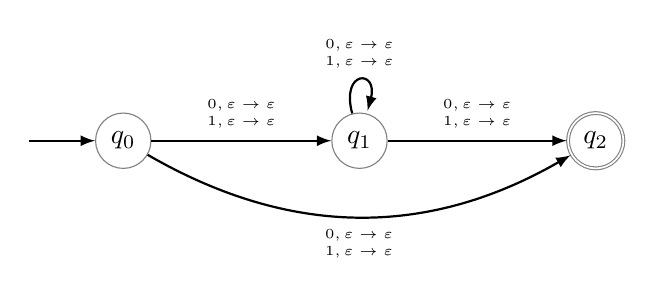
\begin{tikzpicture}[state/.style={circle, draw=black!50, inner sep=0pt, minimum size=20pt},node distance=3cm, on grid, auto] 
		\node[state] (q0) {$q_0$};++
		\node[state] (q1) [right= of q0] {$q_1$};
		\node[state, accepting] (q2) [right=of q1] {$q_2$};
		\draw[<-, thick] (q0) -- ++(-1.2cm,0);
		\path[->,thick] 
			(q0) edge node {\tiny\begin{tabular}{c}$0,\varepsilon \rightarrow \varepsilon$ \\ $1,\varepsilon \rightarrow \varepsilon$ \end{tabular}} (q1)  edge [bend right] node [below] {\tiny\begin{tabular}{c}$0,\varepsilon \rightarrow \varepsilon$ \\ $1,\varepsilon \rightarrow \varepsilon$ \end{tabular}} (q2)
			(q1) edge node {\tiny\begin{tabular}{c}$0,\varepsilon \rightarrow \varepsilon$ \\ $1,\varepsilon \rightarrow \varepsilon$ \end{tabular}} (q2) edge [loop above] node {\tiny\begin{tabular}{c}$0,\varepsilon \rightarrow \varepsilon$ \\ $1,\varepsilon \rightarrow \varepsilon$ \end{tabular}} (q1);
	\end{tikzpicture}
	\end{center}
\newpage
	% \leavevmode \\
	\item[\textbf{c}.] $\{ w \mid $ the length of $w$ is odd$\}$ \\
	\leavevmode \\
	Informal Description: The stack is not needed here at all. Therefore we will read the input and only accept if the length is odd, that is after the first symbol read or every other symbol read thereafter if it is the final symbol read. \\
	\leavevmode \\
	State diagrams: \\
	\begin{center}
	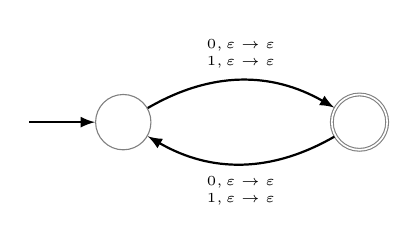
\begin{tikzpicture}[state/.style={circle, draw=black!50, inner sep=0pt, minimum size=20pt},node distance=3cm, on grid, auto] 
		\node[state] (q0) {};
		\node[state, accepting] (q1) [right=of q0] {};
		\draw[<-, thick] (q0) -- ++(-1.2cm,0);
		\path[->,thick] 
			(q0) edge [bend left] node {\tiny\begin{tabular}{c}$0,\varepsilon \rightarrow \varepsilon$ \\ $1,\varepsilon \rightarrow \varepsilon$ \end{tabular}} (q1)
			(q1) edge [bend left] node {\tiny\begin{tabular}{c}$0,\varepsilon \rightarrow \varepsilon$ \\ $1,\varepsilon \rightarrow \varepsilon$ \end{tabular}} (q0);
	\end{tikzpicture}
	\end{center}


	\item[\textbf{e}.] $\{ w \mid w^R$, that is, $w$ is a palindrome$\}$ \\
	\leavevmode \\
	Informal Description: We begin by pushing the symbols read onto the stack. At each point we will nondeterministically guess if the middle of the string has been reached or if the next symbol read is the middle of the string and will not be put on the stack. Then we pop off the symbols from the stack if they match the input symbols read. If the symbols popped are exactly the same symbols that were pushed on earlier and the stack empties as the input is finished, then accept. Otherwise, reject.\\

	\leavevmode \\
	State diagrams: \\ 
	\begin{center}
	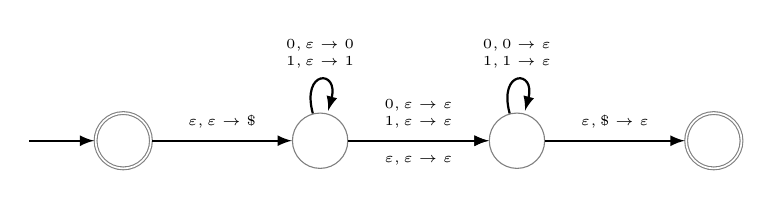
\begin{tikzpicture}[state/.style={circle, draw=black!50, inner sep=0pt, minimum size=20pt},node distance=2.5cm, on grid, auto] 
		\node[state,accepting] (q0) {};
		\node[state] (q1) [right=of q0] {};
		\node[state] (q2) [right=of q1] {};
		\node[state, accepting] (q3) [right=of q2] {};
		\draw[<-, thick] (q0) -- ++(-1.2cm,0);
		\path[->,thick]
			(q0) edge node {\tiny\begin{tabular}{c}$\varepsilon, \varepsilon \rightarrow \$ $ \end{tabular}} (q1)
			(q1) edge [loop above] node {\tiny\begin{tabular}{c}$0,\varepsilon \rightarrow 0$ \\ $1,\varepsilon \rightarrow 1$ \end{tabular}} (q1) edge node {\tiny\begin{tabular}{c}$0,\varepsilon \rightarrow \varepsilon$ \\ $1,\varepsilon \rightarrow \varepsilon$ \end{tabular}} (q2)  edge node [below] {\tiny\begin{tabular}{c}$\varepsilon,\varepsilon \rightarrow \varepsilon$ \end{tabular}} (q2)
			(q2) edge [loop above] node {\tiny\begin{tabular}{c}$0,0 \rightarrow \varepsilon$ \\ $1,1 \rightarrow \varepsilon$ \end{tabular}} (q2) edge node {\tiny\begin{tabular}{c}$\varepsilon,  \$ \rightarrow \varepsilon$ \end{tabular}} (q3);
	\end{tikzpicture}
	\end{center}

	\leavevmode \\
	\item[\textbf{f}.] The empty set \\
	\leavevmode \\
	Note: Since, no derivations terminate, the CFG cannot accept any strings, including the empty. \\
	Informal Description: The PDA consists of one state that does not accept. \\
	\leavevmode \\
	State diagrams: \\ 
	\begin{center}
	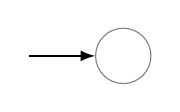
\begin{tikzpicture}[state/.style={circle, draw=black!50, inner sep=0pt, minimum size=20pt},node distance=2.5cm, on grid, auto] 
		\node[state] (q0) {};
		\draw[<-, thick] (q0) -- ++(-1.2cm,0);
	\end{tikzpicture}
	\end{center}
\end{enumerate}

\newpage
%	2.6	%
\item[\textbf{2.6)}] Give context-free grammars generating the following languages.\\
\begin{enumerate}
	\item[\textbf{b}.] The complement of the language \{$a^nb^n \mid n \geq $0\} \\
	\leavevmode \\
	First, we can rewrite the complement as: \\
	\begin{center} $\{a^nb^m$ : $ n \neq m\} \cup \{(a\cup b)^*ba(a \cup b)^*\}$\end{center}
	Let's call the leftmost language $L_1$ and the rightmost $L_2$ \\
	The context-free grammar that generate $L_1$ is: \\
	\setlength\parindent{100pt} 
	$S_1 \rightarrow aS_1b \mid T \ U$ \\
	$T \rightarrow aT \mid a$ \\
	$U \rightarrow Ub \mid b$
	\setlength\parindent{0pt} 

	And for $L_2$ is:\\
	\setlength\parindent{100pt} 
	$S_2 \rightarrow RbaR$ \\
	$R \rightarrow \mid a \mid b \mid \varepsilon$\\
	\setlength\parindent{0pt} 
	So, the final context-gree grammar G that generate $L_1 \cup L_2$ is: \\
	\leavevmode \\
	\setlength\parindent{100pt} 
	$S \rightarrow T \mid aU \mid Vb $\\
	$T \rightarrow aT \mid Ta \mid bT \mid Tb \mid ba$ \\
	$U \rightarrow aU \mid W$\\
	$V \rightarrow Vb \mid W$\\
	$W \rightarrow aWb \mid \varepsilon$\\
	\setlength\parindent{0pt} 


	\item[\textbf{d}.] $\{ x_1\#x_2\#...\#x_k \mid k \geq1$, each $x_i \in \{a,b\}^*$, and for some $i$ and $j$, $x_i = x_i^R\}$ \\
	\leavevmode \\
	First, we can viewed as: \\
	\begin{center} $...\#...\#w\#...\#w^R\#...\#...$\end{center}
	\leavevmode \\
	Let A be a non-terminal that generates $\{a, b, \#\}^*$, i.e.\\
	\leavevmode \\
	\begin{center} $A \rightarrow aA \mid bA \mid \#A \mid \varepsilon$\end{center}
	Then, the part $w\#...\#w^R$ can be generated as follows.\\
	\leavevmode \\
	\begin{center} $B \rightarrow aBa \mid bBb \mid \# \mid \#A\#$\end{center}
	\leavevmode \\
	And then, the context-free grammars that generates is as follows: \\
	\leavevmode \\
	\setlength\parindent{100pt} 
	$S \rightarrow A\#B\#A \mid B\#A \mid A\#B \mid B$\\
	$B \rightarrow aBa \mid bBb \mid \# \mid \#A\#$ \\
	$A \rightarrow aA \mid bA \mid \#A \mid \varepsilon$
	\setlength\parindent{0pt} 
\end{enumerate}

\newpage
%	2.9	%
\item[\textbf{2.9)}] Give a context-free grammar that generates the language.\\
\begin{center} $A = \{a^ib^jc^k \mid i = j or j = k$ where $i, j, k \geq 0 \}$. \end{center}
\leavevmode \\  \leavevmode \\ 
 Is your grammar ambigous? Why or why not? \\
\leavevmode \\
Rules: \\
\tab $S\:\rightarrow\:U\:|\:V$ \\
\tab $U\:\rightarrow\:aU\:|\:X$ \\
\tab $V\:\rightarrow\:Vc\:|\:Y$ \\
\tab $X\:\rightarrow\:bXc\:|\:\varepsilon$ \\
 \tab $Y\:\rightarrow\:aYb\:|\:\varepsilon$ \\ 
\leavevmode \\ 
 The grammar is ambiguous because we can have these two derivations. \\ 
\begin{center}
	\begin{tikzpicture}[tlabel/.style={pos=0.4,right=-1pt,font=\footnotesize\color{red!70!black}}]
	\node{S} 
		child { node{U} 
			child { node{a} }
				child { node{U}
					child { node{X}
						child { node{b} 
						}
						child { node{X} 
							child { node{$\varepsilon$} 
							}
						}
 						child {node{c} 
					}
				}
			}
               	 };
	\end{tikzpicture}
	\begin{tikzpicture}[tlabel/.style={pos=0.4,right=-1pt,font=\footnotesize\color{red!70!black}}]
	\node{S}
		child { node{V} 
			child { node{V} 
				child { node{Y}
					child { node{a} 
					}
				child { node{Y}
                                		child { node{$\varepsilon$}
					}
                           		}
                           		 child { node{b} 
				}
			}
		}
                   		child { node{c} 
			}
               	};
        \end{tikzpicture}
\end{center}


%	2.10	%
\item[\textbf{2.10)}] Give an informal description of a pushdown automaton that recognizes the language $A$ in Exercise 2.9.\\
\leavevmode \\ 
Informal description of a pushdown automaton that recognizes the langauge $A$.\\
\begin{itemize}
	\item Nondeterministically branch to either step 2 or step 6.
	\item Read and push a's.
	\item Read b's, while popping a's.
	\item If b's finish when stack is empty, skip c's on input and $accept$.
	\item Skip a's on input.
	\item Read and push b's.
	\item Read c's, while popping b's.
	\item If c's finish when stack is empty, $accept$.
\end{itemize}
\leavevmode \\ 

%	2.11	%
\item[\textbf{2.11)}] Convert the CFG $G_4$ given in Exercise 2.1 to an equivalent PDA, using the procedure given in Theorem 2.20.\\
\setlength\parindent{150pt} $E \rightarrow E + T \mid T $ \\ $T \rightarrow T \times F \mid F $ \\ $F \rightarrow (E)  \mid  a$ \\  \setlength\parindent{0pt}
\leavevmode \\
	 The formal definition of the equivalent PDA =	(Q, $\Sigma$, $\Gamma$, $\delta$, q$_{1}$, F) where" \\
	Q = \{q$_{1}$,q$_{2}$\}; $\Sigma$ = \{+, x, (, ), a\}\\$\Gamma$ = \{E, T, F\} $\cup$ $\Sigma$; F = \{q$_{2}$\}.\\
	The transition function $\delta$: Q x $\Sigma _{\varepsilon}$ x $\Gamma_{\varepsilon} \longrightarrow$ P(Q X $\Gamma_{\varepsilon}$)\\
	\[   
	\delta(q,x,y) = 
	\begin{cases}
	\text{\{(q$_{2}, \varepsilon$)\}} 
	&\quad\text{if q = q$_{1}$, x = $\varepsilon$}, y =  $\textdollar$ \\
	
	\text{\{(q$_{1}, E+T$), (q$_{1}$, T)\}} 
	&\quad\text{if q = q$_{1}$, x = $\varepsilon$}, y = E \\
	
	\text{\{(q$_{1}, TxF$), (q$_{1}$, F)\}} 
	&\quad\text{if q = q$_{1}$, x = $\varepsilon$}, y = T \\
	
	\text{\{(q$_{1}, (E)$), (q$_{1}$, a)\}} 
	&\quad\text{if q = q$_{1}$, x = $\varepsilon$}, y = F \\
	
	\text{\{(q$_{1}, \varepsilon$)\}} 
	&\quad\text{if q = q$_{1}$, x = y}\\ 
	\end{cases}
	\]	

%	2.12	%
\item[\textbf{2.12)}] Convert the CFG $G$ given in Exercise 2.3 to an equivalent PDA, using the procedure given in Theorem 2.20.\\
\begin{enumerate}
	\item The formal definition of the equivalent PDA\\
	(Q, $\Sigma$, $\Gamma$, $\delta$, q$_{1}$, F)\\
	Q = \{q$_{1}$,q$_{2}$\}; $\Sigma$ = \{a,b\}\\$\Gamma$ = \{R, S, T, X\} $\cup$ $\Sigma$; F = \{q$_{2}$\}.\\
	The transition function $\delta$: Q x $\Sigma _{\varepsilon}$ x $\Gamma_{\varepsilon} \longrightarrow$ P(Q X $\Gamma_{\varepsilon}$)\\
	\[ \delta(q,x,y) = 
	\begin{cases}
	\text{\{(q$_{2},\varepsilon$)\}} 
	&\quad\text{if q = q$_{1}$, x = $\varepsilon$}, y =  $\textdollar$ \\
	
	\text{\{(q$_{1},XRX$),(q$_{1}$,S)\}} 
	&\quad\text{if q = q$_{1}$, x = $\varepsilon$}, y = R \\
	
	\text{\{(q$_{1},aTb$),(q$_{1}$, bTa)\}} 
	&\quad\text{if q = q$_{1}$, x = $\varepsilon$}, y = S \\
	
	\text{\{(q$_{1},(XTX)$), (q$_{1}$, X), (q$_{1}, \varepsilon$)\}} 
	&\quad\text{if q = q$_{1}$, x = $\varepsilon$}, y = T \\
	
	\text{\{(q$_{1}, a$), (q$_{1}$, b)\}} 
	&\quad\text{if q = q$_{1}$, x = $\varepsilon$}, y = X \\
	
	\text{\{(q$_{1},\varepsilon$)\}} 
	&\quad\text{if q = q$_{1}$, x = y}\\ 
	\end{cases}
	\]	
\end{enumerate}

\newpage
%	2.13	%
\item[\textbf{2.13)}]
\begin{enumerate}
	\begin{enumerate}
	\item[\textbf{a.}]
	$L(G)$ is the set of strings that consists of zeros and \#s that either have only 2 \#s and any number of zeros or zeros separated by a single \# and the number of zeros to the right of the \# is double the number of zeros to the left. \\

	\item[\textbf{b.}] $L(G)$ is not regular. This can be proven (by contradiction) by instersecting $L(G)$ with the set of strings of the form 0*\#0*. For instance, \\
	\leavevmode \\
	\tab $A= L(G)\ \bigcap 0^*\#0^*$\\
	\leavevmode \\
	If we assume L(G) is regular, then A must also be regular. \\

	\tab \textit{Let p be the pumping length for A.} \\ 
	\leavevmode \\
	Then the string $w=0^p\#0^{2p}$ is equal to xyz where the absolute value of xy $\leq $ p, y is not the empty string, and $ xy^{i}z $ is an element of $L(G)$ for any i $ \geq $ 0  \\
	\leavevmode \\
	If $x$ contains '\#', then $y$ is to the right of \#. Pumping down would make the number of zeros on the right less than the number of zeros on the left. The resulting string does not belong to $A$. \\
	\leavevmode \\
	If $y$ contains '\#', then pumping $y$ would make the string contain no \#'s. The resulting string does not belong to $A$. \\
	\leavevmode \\
	If $z$ contains '\#'. then again pumping y makes the number of zeros on the right more than twice the amount of zeros on the left. The resulting string does not belong to $A$. \\
	\leavevmode \\
	\textbf{Since A fails the pumping lemma, A is not regular. And therefore, neither is L(G).} \\
	\end{enumerate}
\end{enumerate}


%	2.14		%
\item[\textbf{2.14)}] Convertthe folloing CFG into an equivalent CFG in Chomsky normal form, using the procedure given in Theeorem 2.9.\\
	\tab \tab $A \rightarrow BAB \mid B \mid \varepsilon$ \\
	\tab \tab $B \rightarrow 00 \mid \varepsilon$ \\
\textbf{Solution:} \\
	\tab $S_0 \rightarrow BA_1 |BA|AB|UU|BB| \varepsilon $ \\ 
	\tab $A \rightarrow BA_2 | BA |AB |UU |BB $ \\
	\tab $B \rightarrow UU $ \\ 
	\tab $U \rightarrow 0 $ \\ 
	\tab $A_1 \rightarrow AB $ \\
	\tab $A_2 \rightarrow AB $ \\

\newpage
%	2.26		%
\item[\textbf{2.26)}] Show that if $G$ is a CFG in Chomsky normal form, then for any string $w \in L(G)$ of length $n \geq 1$, exactly $2n - 1$ steps are required for any derivation of $w$ \\
\begin{enumerate}
	\item[]
	\textbf{Lemma:} For all $n \geq 1$, if $G$ derives a sentential form $w$ in $n$ steps, then $n=2T(w) + NT(w) - 1$, where $NT(w)$ is the number of nonterminals in $w$ and $T(w)$ is the number of terminals in $w$. \\
	\leavevmode \\
	This give the desired result as the special case where $w$ has no nonterminals. \\
	\leavevmode \\
	Proof by induction: \\
	\leavevmode \\
	Base case: $n=1$, and deriving $w$ must give one of two forms: $S \Rightarrow a$, where $S \rightarrow A$ is a rule of $G$ and $w = e$. \\
	\tab or:\\
	$S \Rightarrow AB$ where $S \rightarrow AB$ is a rule of $G$ and $w = AB$. \\
	\leavevmode \\
	In the case of the first form $2T(w) + NT(w) -1 = 2  + 0 - 1 = n$, and in the second case, $2T(w) + NT(w) - 1 = 0 + 2 - 1 = n$. \\
	\leavevmode \\
	Induction step:  \\
	\tab $n = 2T(w) + NT(w) - 1$\\
	\tab $n = 2T(x) + NT(x) - 1$  (because $S \Rightarrow ^nx \Rightarrow w$) \\
	\leavevmode \\
	In first case, \\
	\tab $NT(w)  = NT(x) - 1$ and $T(w) = T(x) + 1$ \\
	This gives: $2T(w) + NT(w) - 1 = 2(T(x) + 1) + (NT(x) - 1) - 1 = 2T(x) + NT(x) = n + 1$ \\ 
	\leavevmode \\
	In second case,\\
	\tab $NT(w) = NT(x) + 1$ \\
	\tab and\\
	\tab $T(w)  = T(x) so 2T(w) + NT(w) - 1 = 2T(x) + NT(w) = n+ 1$ \\ 
	\leavevmode \\
	In both case, $2T(w) + NT(w) - 1 = n + 1$ \\
 \end{enumerate}

%	2.30	%
\item[\textbf{2.30)}] Use the pumping lemma to show that the following languages are not context free.\\
\begin{enumerate}
	\item[\textbf{a.}] \{ $0^n1^n0^n1^n \mid n \geq 0$ \} \\
	\leavevmode \\
	\textbf{Solution:} \\
	Strings in $L$ consist of four consecutive \textit{segments}: a zero segment followed by a one segment followed by another zero segment followed by another one segment. Assume that $L$ is context-free and let $p$ denote the pumping length of $L$. Consider the string $0^p1^p0^p1^p \in L$. We can write this string as $uvxyz$ where $|vxy| \leq p$ and $|vy| > 1$. We look at two cases: \\
	\leavevmode \\
	\leavevmode \\
	\underline{\textit{Case 1}}: Either $v$ or $y$ contains more than one type of character ($i.e$. at least one of $v$ and $y$ contains both zeros and ones). In this case, pumping up once to $uv^2xy^2z$ inserts an extra $0^i1^j$ sequence into $s$-$i.e$. the resulting string will contain at least 3 zero segments and 3 one segments. For instance, if $v = 0011$, then pumping once would result in an additional 00 segment followe d by an additional 11 segment. But, strings in $L$ contain only four segments. \\
	\leavevmode \\
	\underline{\textit{Case 2}}: Both $v$ and $y$ contain only one type of character ($i.e$. they are both all zeros or all ones). Since $vxy \leq p$, $vxy$ contains letters from at most 2 segments of $s$. Pumping once to $uv^2xy^2z$ increases the number of characters in one or two of the segments, but leaves the remaining segments untouched. Thus, the number of characters in each segment will be unbalanced.

	\leavevmode \\
	\leavevmode \\
	\item[\textbf{d.}] \{$t_1\#t_2\#...\#t_k \mid k \geq 2$, each $t_1 \in $\{$a,b$\}$^*$, and $t_it_j$ for some $i \neq j$\} \\
	\leavevmode \\
	\textbf{Solution:} \\
	Assume $L$ is context-free and let $p$ denote its pumping length. Consider $s = 0^p1^p\#0^p1^p \in L$. By the pumping lemma, we can write $s$ as $uvxyz$ where $|vxy| \leq p$ and $|vy| > 1$. \\
	\leavevmode \\
	Suppose $vxy$ lies entirely on one side of the \# symbol. Then, pumping once to $uv^2xy^2z$ results in a string where $t1 \neq t2$, so $uv^2xy^2z \notin L$. \\
	\leavevmode \\
	Suppose that $vxy$ contains the \# symbol. If either $v$ or $y$ contains the \# symbol, than we can pump $s$ down to $uv^0xy^0z$, which will not contain the \# symbol and hence will not be in $L$. Otherwise, the \# symbol is contained in $x$, $v$ is a substring of $1^p$, and $y$ is a substring of $0^p$ (since $|vxy| \leq p$). Pumping $s$ down to $uv^0xy^0z$ reduces either the number of ones in $t_1$ or the number of zeros in $t_2$ or both. As a result, $t1 \neq t2$ for $uv^0xy^0z$, so the string is not in $L$.
 \end{enumerate}

\newpage
%	2.31	%
\item[\textbf{2.31)}] Let B be the language of all palindromes over $\{0,1\}$ containing equal numbers of 0s and 1s. Show that B is not context free.\\
\leavevmode \\
\textbf{Solution:} \\
\begin{itemize}
	\item[--] We assume that $B$ is a Context Free Langauge and obtain a contradiction.
	\item[--] Let $p$ be the pumping constant of $B$ that is quaranteed to exist by the pumping lemma. Select the string $s=0^p1^p1^p0^p$.
	\item[--] Clearly $\textbf{s}$ is a member of $B$ and of length at least $p$ . We can show that no matter how we divide $\textbf{s}$ into $uvxyz$, one of the conditions of the lemma is violated.
	\begin{itemize}
		\item Pumping lemma, $|vxy| \leq p$ , we can only place $vxy$ in the following ways:
		\begin{enumerate}
			\item[1.] $vxy$ completely falls in the first $0^p$ (If we pump $v$ and $y$ , then the new string is no longer a palindrome, and the number of 0s will be greater than the number of 1s, which is a contradiction). \\
			
			\item[2.] $vxy$ falls between $0^p$ and $1^p$ (In this case, $v$ will only contain 0s while $y$ will only contain 1s. So if we pump $s$ , the new string is no longer palindrome, which is a contradiction). \\

			\item[3.] $vxy$ completely falls in the first $1^p$ (Similar to (1), after pumping $s$ , the number of 1s will be greater than the number of 0s, which is a contradiction). \\

			\item[4.] $vxy$ falls between $1^p$ and $1^p$ (After pumping $s$ , the number of 1s will be greater than the number of 0s, which is a contradiction). \\

			\item[5.] $vxy$ completely falls in the second $1^p$ (This case is same with (3)). \\ 

			\item[6.] $vxy$ falls between $1^p$ and $0^p$ (Similar to (2), v will only contain 1s while $y$ will only contain 0s. So if we pump $s$ , the new string is no longer palindrome, which is a contradiction). \\

			\item[7.] $vxy$ completely falls in the second $0^p$  (This case is same with (1)). \\

		\end{enumerate}
	\end{itemize}
\end{itemize}
Hence, $B$ is not context free.

\newpage

%	2.32		%
\item[\textbf{2.32)}] Let $\sum = \{1, 2, 3, 4\}$ and $C = $\{$w \in \sum * |$ in $w$, the number of 1s equals the number of 2s, and the number of 3s equals the number of 4s \}. Show that $C$ is not context free. \\
\leavevmode \\
\textbf{Solution:} \\
$C =$\{$w \in$ \{$0, 1, 2, 3, 4$\}$^* \mid $ in $w$ the number of 1s equals the number of 2s and the
number of 3s equals the number of 4s \} \\

\leavevmode \\
For a contradiction assume that $C$ is context free. Therefore, $C$ has a pumping length $p$. Take $s = 1^p3^p2^p4^p \in C$ with $|s| > p$. Therefore, there exists $uvxyz$ such that (1) $uv^ixy^iz \in C$ for all $i \geq 0$, (2) $|vy| > 0$ and (3) $|vxy| \leq p$. We will now proceed by cases to show that no matter the values of $uvxyz$ we choose, we will reach a contradiction. \\

\leavevmode \\
\underline{\textit{Case 1}}: $vxy$ contains a 1. Then $uv^2xy^2z \notin C$, since it will no longer have the same number of 1s and 2s. This is because from (3), $vxy$ cannot contain any 2s. \\

\leavevmode \\
\underline{\textit{Case 2}}: $vxy$ contains a 2. Then $uv^2xy^2z \in C$, since it will no longer have the same number of 1s and 2s. This is because from (3), $vxy$ cannot contain any 1s. \\

\leavevmode \\
\underline{\textit{Case 1}}: $vxy$ contains a 3. Then $uv^2xy^2z \in C$, since it will no longer have the same number of 3s and 4s. This is because from (3), $vxy$ cannot contain any 4s. \\

\leavevmode \\
\underline{\textit{Case 1}}: $vxy$ contains a 4. Then $uv^2xy^2z \in C$, since it will no longer have the same number of 3s and 4s. This is because from (3), $vxy$ cannot contain any 3s. \\

\leavevmode \\
From (2) we see that these are all the cases. In each one we contradict (1). Therefore, $C$ is not context free.


\newpage
%	2.47 	%
\item[\textbf{2.47)}] Let  $\Sigma$= $\{0,1\}$ and let $B$ be the collection of strings that contain at least one 1 in their second half. In other words, $B$ = $\{\textit{uv} | \textit{u} \in \Sigma^*, \textit{v} \in \Sigma^*1\Sigma^* and |\textit{u}| \geq |\textit{v}|\}$ \\

\item[\textbf{a}.] Give a PDA that recognizes $B$. \\
The PDA M that recognizes $B$ is ($Q$, $\Sigma$, $\Gamma$, $\delta$, $q_0$, $F$), where: \\
	\tab \tab $Q$ = \{$q_0$, $q_1$, $q_2$, $q_3$\},\\
	\tab \tab $\Sigma$ = \{0, 1\}, \\
	\tab \tab $\Gamma$ =\{x\} \\
	\tab \tab $F$ = \{$q_3$\} \\
Transition function $\delta$ is presented as the following state diagram for the PDA:\\
	\begin{center}
	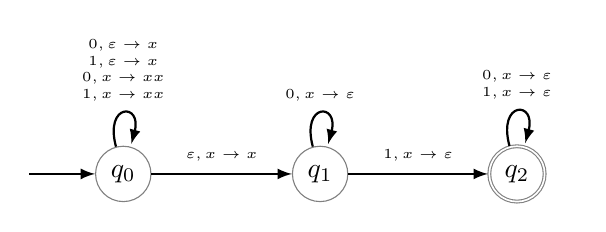
\begin{tikzpicture}[state/.style={circle, draw=black!50, inner sep=0pt, minimum size=20pt},node distance=2.5cm, on grid, auto] 
		\node[state] (q0) {$q_0$};
		\node[state] (q1) [right=of q0] {$q_1$};
		\node[state, accepting] (q2) [right=of q1] {$q_2$};
		\draw[<-, thick] (q0) -- ++(-1.2cm,0);
		\path[->,thick]
			(q0) edge [loop above] node {\tiny\begin{tabular}{c}
				$0,\varepsilon \rightarrow x$ \\
				$1,\varepsilon \rightarrow x$ \\
				$0, x \rightarrow xx$\\
				$1, x \rightarrow xx$\end{tabular}}
			(q0) edge node {\tiny\begin{tabular}{c}$\varepsilon, x \rightarrow x $ \end{tabular}} (q1)
			(q1) edge [loop above] node {\tiny\begin{tabular}{c}$0,x \rightarrow \varepsilon$ \end{tabular}} 
			(q1) edge node {\tiny\begin{tabular}{c}$1, x \rightarrow \varepsilon$\end{tabular}}(q2) 
			(q2) edge [loop above] node {\tiny\begin{tabular}{c}$0,x \rightarrow \varepsilon$ \\
											$1,x \rightarrow \varepsilon$ \end{tabular}} (q2);
	\end{tikzpicture}
	\end{center}
\item[\textbf{b}.]CFG is: \\
		\leavevmode \\
	\setlength\parindent{100pt} 
	$S \rightarrow UV$\\
	$U \rightarrow AB$ \\
	$V \rightarrow A1A \mid A1B \mid A1U \mid B1U \mid U1U$\\
	$A \rightarrow 00^* \mid \varepsilon$\\
	$W \rightarrow 11^* \mid \varepsilon$\\
	\setlength\parindent{0pt} 

Explanation:\\
	\begin{itemize}
		\item The string $S$ is the concatenation of $U$ and $V$.
		\item The string $U$ may consist of any number of 0's and 1's.
		\item The string $V$ may consist of at least one 1 or only one 1.
		\item The string $A$ may consist of at least one zero or more than one zeros
		\item The string $B$ may consist of at least one 1 or more than one 1.
	\end{itemize}

\newpage
\tab \tab \tab Extra Credit \\
\leavevmode \\
\leavevmode \\

%	2.20 	%
\item[\textbf{2.20)}] Let $A/B$ = \{ $w| wx \in A$ for some $x \in B$ \}. Show that if $A$ is context free and $B$ is regular, then $A/B$ is context free.

Suppose $A$ is context-free and $B$ is regular. Let \\
\leavevmode \\
	\tab \tab $P = (Q_P , \Sigma, \Gamma_P , \delta_P , q_0,P , F_P)$ \\
\leavevmode \\
	\tab \tab be a PDA that recognizes $A$, and let \\
\leavevmode \\
	\tab \tab $M = (Q_M, \Sigma, \delta_M, q_0,M, F_M)$ \\

be a NFA that recognizes $B$. We will show that $A/B$ is context-free by constructing a PDA $P' = (Q', \Sigma, \Gamma', \delta', q'_0, F')$ that recognizes A/B.\\
\leavevmode \\
\tab The intuitive idea of the construction is as follows: $P'$ will start out behaving like $P$ while reading a prefix $w$ of the input string. At a nondeterministically chosen point, $P'$ will "guess" that it has reached the end of $w$. At this point, it will behave like $P$ and $M$ running simultaneously, except that it will "guess" the input string $x$, rather than actually reading it as input. If it is possible in this way to simultaneously to reach an accepting state of both $P$ and $M$, then $P'$ accepts. Note that there is no reason why the stack would have to be empty at the point where $P'$ begins the guessing phase. So it is necessary for $P'$ to continue simulating $P$, in order to properly account for the stack contents.\\
\leavevmode \\
\tab Formally, we define $P'$ as follows: \\
	\begin{itemize}
	\item $Q' = Q_b \cup (Q_p \times Q_M)$
	\item $\Gamma' = \Gamma$
	\item $q'_0 = q_{0,P}$
	\item $F' = F_P \times F_M$
	\item $\delta'$ is defined as follows: For $q_P \in Q_P$ ($i.e$. if $P$ is in the initial phase): \\
	\[  \delta (q_P,x,y) = 
		\begin{cases}
			\text{$\delta_P(q_P,a, u$)}  &\quad\text{$if a \in \Sigma$ } \\
	
			\text{$\delta_P(q_P,\empty, u) \cup \{(q_P, q_{M,0}), \empty $\}} 	&\quad\text{if $a \in \empty$.}\\
		\end{cases}
	\]

	\item For $(q_P, q_M) \in Q_P \times Q_M$ ($i.e.$ if $P'$ is in the guessing phase): \\
	\[  \delta'((q_P,q_M),a,u) = 
		\begin{cases}
			\text{$\emptyset$ } , \text{if $a \in \Sigma$.}\\
	
			\text{$\cup_{b \in \Sigma_{\empty}}$ \{$((r_P,r_M), v) $  $: (r_P, v) \in \delta_P(q_P,b,u)$ and $r_M \in \delta_M(q_M,b)$\} } , \text{if $a \in \empty$.}\\
		\end{cases}
	\]

	\end{itemize}
	 We claim that $P'$ accepts $w$ if and only if there exists a string $x$ such that $P$ accepts $wx$ and $M$ accepts $x$. For, in an accepting computation of $P'$ on input $w$, all of $w$ must be read during the first phase (since nothing is read during the guessing phase), and the input symbols $b$ that are guessed during the second phase determine a string $x$ that is accepted by $M$ and is such that $wx$ is accepted by $P$. Conversely, if $w$ is a string with the property that $wx \in A$ for some $x \in B$, then there is an accepting computation of $P'$ in which $w$ is read during the first phase, and then the input $x$ is guessed during the second phase. In this case, the P-components of the states determine an accepting computation of P on input $wx$, and the M-components of the states determine an accepting computation of $M$ on input $x$.



%	2.36 	%
\item[\textbf{2.36)}] Give an example of a language that is not context free but that acts like a CFL in the pumping lemma. Prove that your example works. \\
\leavevmode \\
 \begin{enumerate}
\item[] Consider the language $F = {a^ib^jc^k \mid i,j,k \geq 0 \text{ and if } i = 1 \text{ then } j = k}$.  It is not a CFL because it is not a regular language (see Exercise 1.54). But it can be pumped like a CFL in the case where $i > 1$.  \\
\begin{proof}
	\mbox{}
	\begin{itemize}
	  \item Let $s = a^i b^j c^k = uvxyz$.
	  \item If $u = a^i$ and $z = c^k$, then $s$ can be pumped, giving $uv^ixy^iz$,
	  where $v^ixy^i$ is an expanding series of $b$s.
	\end{itemize}
\end{proof}
\end{enumerate}


%	2.44 	%
\item[\textbf{2.44)}] If $A$ and $B$ are languages, define $A \diamond B = $ \{ $xy \mid x \in A \text{ and } y \in B \text{ and } |x| = |y| $ \}. Show that if $A$ and $B$ are regular languages, then $A \diamond B$ is a CFL. \\
\leavevmode \\
 \begin{enumerate}
\item[] To satisfy the condition that $|x| = |y|$, the use of a stack is required when building a machine to recognize $A \diamond B$. A stack cannot be used in a DFA or NFA, but it can be used in an PDA. Thus, $A \diamond B$ can only be recognized by an PDA. By lemma 2.27 in Sipser, if a PDA recognizes a language, then that language is a CFL. Thus, $A \diamond B$ is a CFL.
\end{enumerate}










































\end{enumerate}
\end{document} 